%\section{Discussion}


\subsection{Comparison of beading schemes}
We can see from \cref{TEST_naive_accuracy}(top) and~\ref{over_underfill} that the uniform technique causes a lot of overfills and underfills: on average approximately \SI{1}{\percent} of the total target area is covered by underfill and likewise for overfill.
These defects are supposed to negatively influence the mechanical properties of the parts, and exceed the point that process parameters can be reliably correlated to mechanical properties of the part. 
To our knowledge, the uniform beading scheme, as well as the outer beading scheme, is of little use to FDM printers.

The constant bead count scheme effectively deals with underfills, but generates orders of magnitude more overfills compared to the other schemes. 
Also, the scheme comes at the cost of greatly varying bead widths and an average bead width that is not close to the nominal bead width.
Note that most overfill areas occur near regions of alternating bead width. 
For an input outline shape which contains both very small and very large features, the the constant bead count scheme produces bead widths which can fall outside of the range of manufacturable bead widths.
Moreover the centrality marking is not robust against small perturbations in the outline; adding a small chamfer in a corner causes the unmarked ST to be very small at that location, which results in tiny bead widths.

In \cref{TEST_Center_accuracy} we can see that
the centered beading scheme effectively deals with both overfill and underfill and produces desired bead widths in all locations, except for the extrusion paths in the center, where the bead widths are within a factor 2 off from the desired bead width.
According to \cref{over_underfill} the overfill and underfill for the centered, the evenly distributed and the inward distributed scheme are all approximately \SI{0.2}{\percent}, which is a considerable improvement over the uniform technique.

However, according to \cref{widthHistogram} the centered scheme exhibits a wider range of bead widths than the distributed schemes:
the standard deviation of the bead widths in the centered scheme is approximately \SI{39}{\micro\meter}, while that of the distributed schemes is approximately \SI{14}{\micro\meter}.
We can therefore state that the distributed schemes result in bead widths closer to the nominal widths compared to the centered scheme.
This is desirable for the manufacturability of the beads and can therefore have a positive effect on the mechanical properties and surface quality of the 3D prints. 

The inward distributed scheme is introduced with the intention to limit the number of beads deviating from the nominal bead width and to limit the number of angled extrusion segments in transitioning regions.
This expected effect is difficult to be confirmed when comparing \cref{TEST_Distributed_accuracy} with~\ref{TEST_InwardDistributed_accuracy}, because there are no large solid areas in that specific shape.

However, when comparing the bead width of the outer toolpaths, \cref{distributed_comparison} and  \cref{widthIndexedHistogram}, we can clearly see that the these toolpaths have the nominal bead width more often, which means that errors from inaccuracies due to deviation from the nominal bead width are concentrated near the center of the shape, leaving the dimensional accuracy of the outline shape less affected, if at all. 
Furthermore, we find that compared to evenly distributed, the inward distributed scheme produces smoother toolpaths overall (\cref{smoothness}), and with less jaggedness on the contour toolpaths (\cref{smoothness}). 
Therefore, when using the inward distributed scheme the surface of the 3D print is less affected by both width variation and jagged toolpaths, while overfill and underfill are kept at a low percentage.


\subsection{Theoretical analysis}
\jun{I suggest to dissolve this subsection. see comments and suggested changes below.}

In this paper the significance measure is not used heuristically, as it is sometimes used in other literature.
The significance measure is an exact measure of the relative size of gaps when using the uniform toolpathing method.
See \cref{naive_overfill_underfill}
\jun{this is in the method, and thus can be removed.}
Note also that contrary to some literature we do not remove edges from the skeleton, but leave it intact.
The final skeleton is still an exact and full feature descriptor.
In that sense our framework provides an exact solution space.
\jun{what is a solution space? what is the benefit of using an exact and full feature descriptor regarding toolpath accuracy, uniformity and smoothness?}

Note also that our method is robust against small perturbations in the input shape.
Geometrically small changes to the outline shape introduce extra edges and therefore change the topology of the graph of the ST.
However, the significance measure and beading are defined in terms of radial distances so the robustness of the distance field against such perturbations means our method bypasses the instability of the skeleton. \jun{this could be mentioned somewhere in the method, shortly. The uniform approach can also be thought of using the distance field, is it less robust than ours?}
Moreover, we have developed a method for dealing with edges within transition regions such that the toolpath is the same as if there was no such edge in that region.
The toolpaths generated using our framework therefore remain the same when extra edges are added to the ST.
\jun{this could be integrated in paragraph Smooth transitions to motivate the fractional bead count}

Our framework is also local.
The toolpathing around some section of the input polygons is independent of far away regions of the polygon.
This means the toolpathing is stable against large perturbations of the input shape in far away regions
and it also allows for some parallelism during the computation of the toolpaths.
\jun{This could mentioned in paragraph Computational performance. This potentially could be parallelized for speeding up.}













\subsection{Applications}
Toolpath with varying width is particularly meaningful for narrow parts, since there the negative effect of under- and overfill is more pronounced than in wide parts.
In extreme cases, thin features will not be filled at all.
Therefore, our framework, while working for wide parts as well, shows most of its potential for objects which contain thin parts.

\Cref{applications_overview} collectively shows the application of the proposed inward distributed scheme for various types of 3D model, including both thin parts (architectural models, casings, embossed text, gears and microstructures) and wide parts (\cref{applications_case}) and organic shapes (\cref{applications_statue})).

For architectural models and casings, preventing over- and underfill is expected to make them stronger. 
For embossed text, preventing underfill reduces the various holes in the top surfaces, which is detrimental to the visual quality of those top surfaces.
For gears and similar mechanical parts that are designed with finite element analysis, the less variation in extrusion widths is closer to the assumptions under fast analysis (e.g. using homogenization~\cite{Liu2016CAD}).

Of particular interest are microstructures that could be uniquely fabricated by 3D printing.
For example, topology optimized bone-like structures~\cite{wu2017infill} contain filaments of varying thickness that follow a varying stress direction (\cref{applications_bone}).
An angled Gyroid structure with uniform thickness also results in outline shapes with varying width (\cref{applications_gyroid}). 
These structures are accurately densely filled using our framework.
Another class of microstructures consists of parameterized patterns with varying thickness to achieve functional gradation.
\Cref{applications_hex} shows the contour-parallel toolpath with varying width of a hexagonal grid neatly switches between different bead counts over the volume, preventing the jagged moves a direction-parallel toolpath would create for such a case~\cite{bates2018compressive}.


\begin{figure*}
\centering
\setlength{\figwidth}{0.099\textwidth}
\setlength{\figheight}{0.099\textwidth}
\begin{subfigure}{\textwidth}\centering
\censorbox{
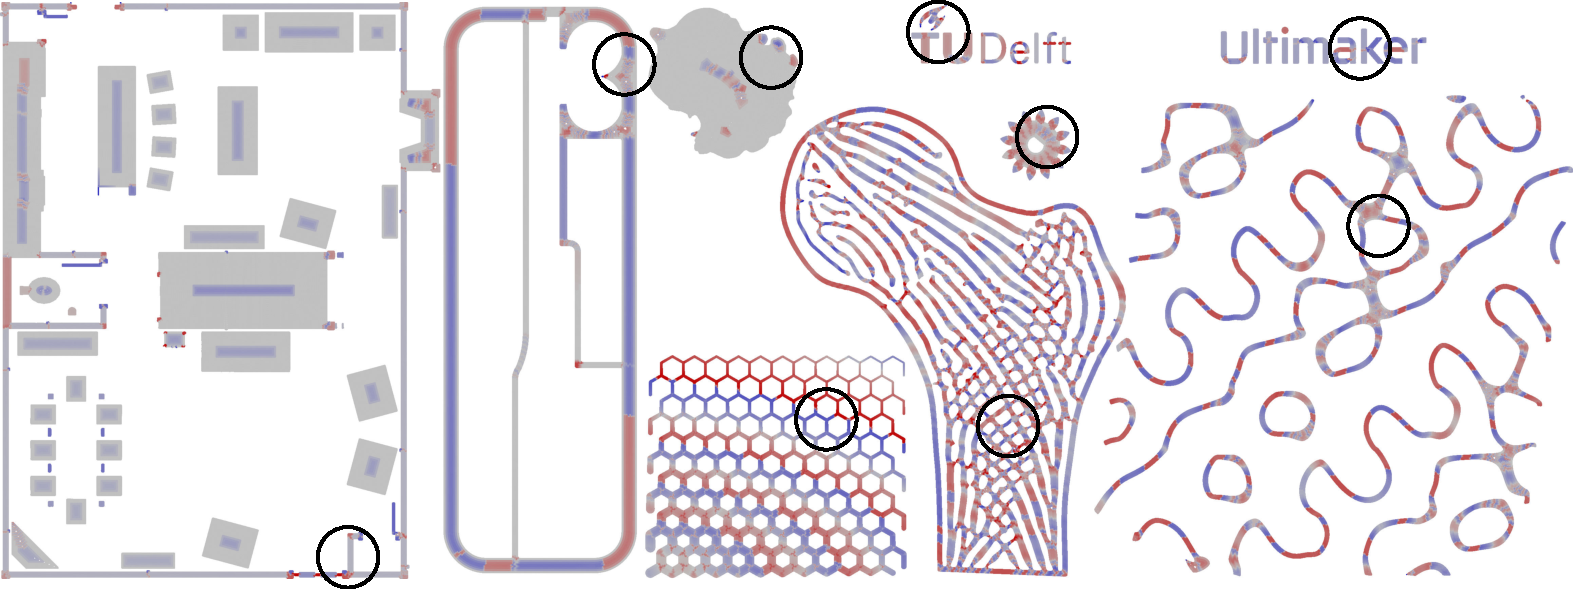
\includegraphics[width=\textwidth]{sources-applications-combined-small-dilated-circled.pdf}
}
%\caption{Overview}\label{applications_overview}
\end{subfigure}
\begin{subfigure}[t]{\figwidth}\centering
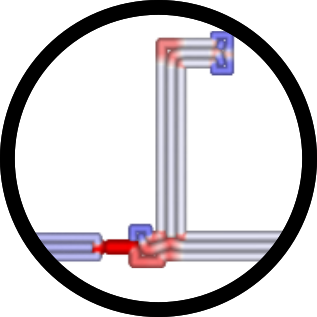
\includegraphics[height=\figheight]{sources-applications-house.png}
\caption{House}\label{applications_house}
\end{subfigure}
\begin{subfigure}[t]{\figwidth}\centering
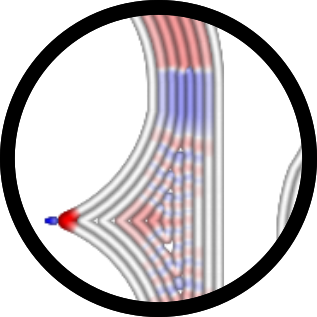
\includegraphics[height=\figheight]{sources-applications-pocket-operator-case.png}
\caption{Case}\label{applications_case}
\end{subfigure}
\begin{subfigure}[t]{\figwidth}\centering
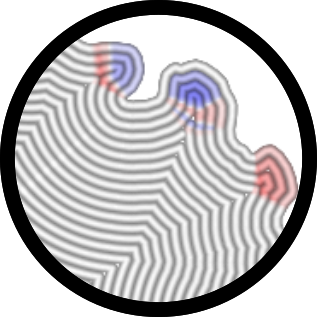
\includegraphics[height=\figheight]{sources-applications-david.png}
\caption{Statue}\label{applications_statue}
\end{subfigure}
\begin{subfigure}[t]{\figwidth}\centering
\censorbox{
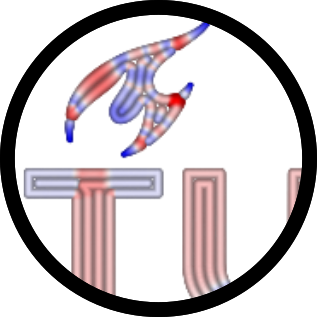
\includegraphics[height=\figheight]{sources-applications-tud-logo.png}
}
\caption{\censor{TUD}}\label{applications_tud}
\end{subfigure}
\begin{subfigure}[t]{\figwidth}\centering
\censorbox{

\includegraphics[height=\figheight]{sources-applications-ultimaker-logo.png}
}
\caption{\censor{UM}}\label{applications_um}
\end{subfigure}
\begin{subfigure}[t]{\figwidth}\centering
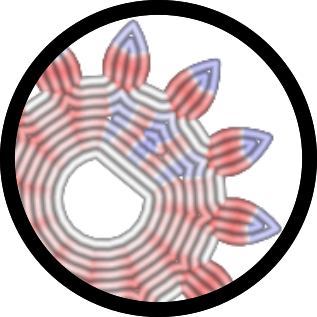
\includegraphics[height=\figheight]{sources-applications-pinion-gear-motor.png}
\caption{Gear}\label{applications_gear}
\end{subfigure}
\begin{subfigure}[t]{\figwidth}\centering
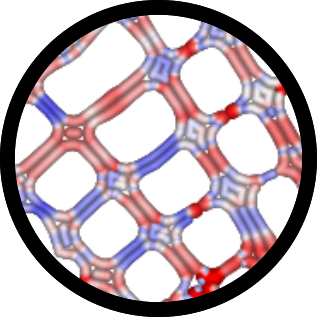
\includegraphics[height=\figheight]{sources-applications-topopt-bone.png}
\caption{Bone}\label{applications_bone}
\end{subfigure}
\begin{subfigure}[t]{\figwidth}\centering
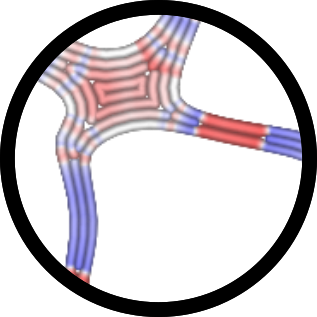
\includegraphics[height=\figheight]{sources-applications-gyroid.png}
\caption{Gyroid}\label{applications_gyroid}
\end{subfigure}
\begin{subfigure}[t]{\figwidth}\centering
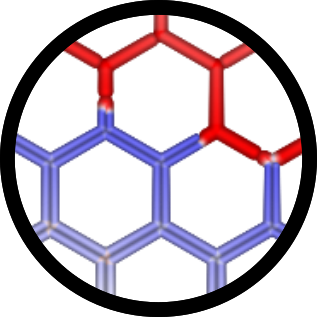
\includegraphics[height=\figheight]{sources-applications-hex-grid.png}
\caption{Hex}\label{applications_hex}
\end{subfigure}
\begin{subfigure}[t]{.3\figwidth}
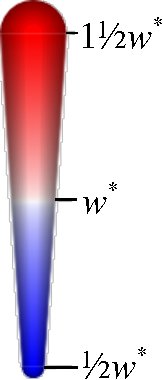
\includegraphics[height=\figheight]{sources-validation-widths-legend-small.pdf}
\end{subfigure}
\caption{
Visualization of the widths for the output toolpaths of the inward distributed beading scheme {($N=3$) }applied to various example application objects.
From left to right and top to bottom: a house, a case for electronics, a statue, two common logos, a gear, a topologically optimized bone structure, a tilted homogeneous gyroid structure and a heterogeneous thickness hexagonal grid.
}
\label{applications_overview}
\end{figure*}














\subsection{Limitations}
Note that the current industry standard in FDM printing employs little to no bead width variation.
Properly performing bead width variation calls for adaptations and developments in printers and firmware.
In the beading schemes we set a transition length of $t(n) = w^*$.
That will demand changes in cross-sectional area of the bead up to \SI{200}{\percent} over a small distance that is comparable to the nozzle size, which is challenging for some hardware systems.
Varying the movement speed can be utilised to change the cross-sectional area, but this approach is limited, since the movement speed is constrained by acceleration considerations near bends in the toolpath.
Our schemes require a more accurate control of the volumetric flow rate in \si{\milli\meter\cubed\per\second}.
Using a filament feeder directly mounted on the print head (a.k.a. direct drive) outperforms Bowden style FDM printers in terms of dynamic flow changes,
but still requires some control system in order to accurately change the volumetric flow rate such as pressure advance algorithms~\cite{tronvoll2019investigating}.
Yet inaccuracies in direct drive systems employing advance algorithms might arise due to the changes in back-pressure required by changing bead size.
We expect that developments in printing hardware and firmware will address these challenges in the future.


Another limiting factor in the adoption of adaptive bead width is the format of G-code which stores machine instructions.
G-code does not support moves with varying cross-sectional area.
A typical extrusion move \lstinline{G1 X$x$ Y$y$ E$v$} only specifies the total amount of volume $v$ to be extruded in the move, not how that total amount should be distributed along the extrusion move.
A workaround is to approximate a variable width extrusion segment by smaller segments with constant width.
However, this introduces errors nevertheless.
Ideally the G-code language would be expanded in some way to allow for extrusion segments with varying cross-sectional area.


% Taking a broader perspective, we note that our proposed inward distributed scheme is a pragmatic solution.
% Rather than deriving some optimal beading scheme from a clear specification of the objective, we propose some arbitrary inward distributed beading scheme and show that it is better than the other beading schemes.
% An optimal beading scheme can be derived if the objective is formalized terms of a unambiguous fitness function, but that would depend on the specific hardware setup and application for which toolpaths are generated.
% This manuscript is therefore limited to showing the flexibility and versatility of the framework, rather than deriving an optimal beading scheme.




